\addcontentsline{toc}{chapter}{Занятие 13. Последовательности случайных величин. Лемма Бореля-Кантелли}
\chapter*{Занятие 13. Последовательности случайных величин. Лемма Бореля-Кантелли}

\addcontentsline{toc}{section}{Контрольные вопросы и задания}
\section*{Контрольные вопросы и задания}

\subsubsection*{Сформулируйте лемму Бореля-Кантелли, закон <<нуля или единицы>> Колмогорова; запишите теоретико-множественное изображение событий $ \varlimsup \limits_{n \to \infty } A_n, \, \varliminf \limits_{n \to \infty } A_n$.}

Лемма Бореля-Кантелли.
\begin{enumerate}
\item Если
$$ \sum \limits_{n=1}^{ \infty } P \left( A_n \right) < + \infty,$$
то $P \left( \varlimsup \limits_{n \to \infty } A_n \right) = 0$;
\item если $ \left\{ A_n \right\} $ --- независимы и
$$ \sum \limits_{n=1}^{ \infty } P \left( A_n \right) =
+ \infty $$
(ряд, составленный из вероятностей, расходится), то $P \left( \varlimsup \limits_{n \to \infty } A_n \right) = 1$.
\end{enumerate}

Закон <<нуля или единицы>> Колмогорова.
Пусть дано вероятностное пространство
$ \left( \Omega, \mathcal{F}, \mathbb{P} \right) $
и определённая на нём последовательность независимыых случайных величин
$ \left\{ X_n \right)_{n=1}^{ \infty } $ (не обязятельно одинаково распределённых).
Пусть $ \mathcal{F}_{ \infty }$ --- её остаточная $ \sigma $-алгебра, то есть
$$ \mathcal{F}_{ \infty } =
\sigma \left( \bigcap \limits_{m=1}^{ \infty } \bigcup \limits_{n \geq m} \mathcal{F}_n \right),$$
где $ \mathcal{F}_n $ есть $ \sigma $-алгебра, порождённая случайной величиной $X_n$.

Тогда если $A \in \mathcal{F}_{ \infty }$, то $ \mathbb{P} \left( A \right) = 0$ или $ \mathbb{P} \left( A \right) = 1$.

Другими словами, $A$ --- остаточное событие, если оно измеримо относительно $ \sigma $-алгебры,
порождённой случайными величинами $ \left\{ X_n \right\}_{n=1}^{ \infty }$, но независимо от любого конечного подмножества этих величин.
Согласно теореме, такое событие имеет вероятность ноль или единица.

Пусть $ \left\{ A_n \right\}_{n \geq 1}$ --- последовательность случайных событий.

$$ \varlimsup \limits_{n \to \infty } A_n =
\bigcap \limits_{n=1}^{ \infty } \bigcup \limits_{m=n}^{ \infty } A_m.$$

Это означает, что $ \forall n \, \exists m, \qquad A_m$ произошло.
В последовательности
$$ \left\{ A_n \right\}_{n \geq 1}$$
происходит бесконечно много событий $A_n$.

$$ \varliminf \limits_{n \to \infty } \bigcup \limits_{n=1}^{ \infty } \bigcap \limits_{m=n}^{ \infty } A_m =$$
= \{начиная с некоторого номера в $ \left\{ A_n \right\}_{n \geq 1}$ происходят все события $A_n$\}.

$ \exists n \, \forall m, \qquad A_m$ произошло.

\addcontentsline{toc}{section}{Аудиторные задачи}
\section*{Аудиторные задачи}

\subsubsection*{13.3}

\textit{Задание.} Найдите вероятность того, что при последовательных подбрасываниях монеты серия из пяти последовательных гербов выпадет бесконечно много раз.

\textit{Решение.}
Введём события $A_1 =$ \{герб выпадет при подбрасываниях 1 --- 5\}, $A_2 =$ \{герб выпадет при подбрасываниях 6 --- 10\},
$\dotsc, \, A_n =$ \{герб выпадет при подбрасываниях $\left( 5 \left( n-1 \right) + 1 \right) - 5n$\}.

Хотим доказать, что ряд из вероятностей таких событий расходится.
Для этого нужно посчитать вероятность такого события.

Подбрасывания независимы
$$P \left( A_k \right) =
\left( \frac{1}{2} \right)^5.$$

Имеем ряд
$$ \sum \limits_{k=1}^{ \infty } P \left( A_k \right) =
+ \infty.$$

По второй части леммы Бореля-Кантелли $P \left( \varlimsup \limits_{n \to \infty } A_n \right) = 1$.

\subsubsection*{13.4}

\textit{Задание.}
Пусть $ \left\{ \xi_n \right\}_{n \geq 1}$ --- последовательность независимых случайных величин,
причём $P \left( \xi_n = 1 \right) = p, \, P \left( \xi_n = 0 \right) = 1 - p$.
Докажите, что
$$P \left( \sum \limits_{n=1}^{ \infty } \xi_n = + \infty \right) = 1.$$

\textit{Решение.} $ \left\{ \xi_n \right\}_{n \geq 1}$ --- независимые случайные величины.

Известно, что $P \left( \xi_n = 1 \right) = p, \, P \left( \xi_n = 0 \right) = 1 - p$.

Нужно показать, что
$$P \left( \sum \limits_{n=1}^{ \infty } \xi_n = + \infty \right) = 1.$$

Если $p = 0$, то ряд сходится.
Поэтому изначально предполагаем, что $p > 0$.

Если бесконечно много единиц, тогда ряд расходится.
Нужно показать,
что в последовательности $ \xi_1, \xi_2, \dotsc, \xi_n, \dotsc $ бесконечно много единиц,
т.е. $P \left( A_n \right.$ бесконечно часто) $= 1, \, A_n = \left\{ \xi_n = 1 \right\} $.

Эти события независимы, потому что $ \left\{ \xi_n \right\} $ --- независимы, $P \left( A_n \right) = p$.

Тогда
$$ \sum \limits_{n=1}^{ \infty } P \left( A_n \right) =
\sum \limits_{n=1}^{ \infty } p =
+ \infty.$$

\subsubsection*{Задача}

\textit{Задание.} Предположим, что игральный кубик подбрасывается бесконечное число раз независимым образом.
На нём 6 граней.
Кубик симметричный.
Доказать, что с вероятностью 1 последовательность из ста двоек встречается бесконечное число раз.

\textit{Решение.}
$$ \xi_n =
\begin{cases}
1, p_1 = \frac{1}{6}, \\
2, p_2 = \frac{1}{6}, \\
3, p_3 = \frac{1}{6}, \\
\dotsc \\
6, p_6 = \frac{1}{6}.
\end{cases}$$

Нужно доказать,
что $P$ \{последовательность $ \left( 2, 2, \dotsc, 2 \right) $, где 100 двоек, выпадает бесконечно часто\} $= 1 = P \left( \varlimsup \limits_{n \to \infty } A_n \right) $.

Введём события $A_1 =$ \{выпадет двойка при первых ста подбрасываниях\}, $A_2 =$ \{выпадет двойка при 101-ом --- 200-ом подбрасываниях\},
$ \dotsc, \, A_n =\\
=$ \{выпадет двойка при $100 \left( n-1 \right) + 1$ --- $100n$ подбрасываниях\}.
Нужно найти вероятность такого события
$$P \left( A_n \right) =
\left( \frac{1}{6} \right)^{100}.$$

Ряд, составленный из этих вероятностей расходится $ \sum \limits_{n=1}^{ \infty } P \left( A_n \right) = + \infty $.

\subsubsection*{13.5}

\textit{Задание.} Пусть $ \left\{ \xi_n \right\}_{n \geq 1}$ --- последовательность независимых случайных величин.
Найдите вероятность $P \left( \varliminf \limits_{n \to \infty } \xi_n = 0 \right) $, если:
\begin{enumerate}[label=\alph*)]
\item $P \left( \xi_n = k/n \right) = 1/n, \qquad k = 1, \dotsc, n$;
\item $P \left( \xi_n = k/n \right) = 2k/\left[ n \left( n+1 \right) \right], \qquad k = 1, \dotsc, n$.
\end{enumerate}

\textit{Решение.}
\begin{enumerate}[label=\alph*)]
\item Есть последовательность независимых случайных величин $ \left\{ \xi_n \right\} $ такая, что
$$P \left\{ \xi_n = \frac{k}{n} \right\} =
\frac{1}{n}, \qquad
1 \leq k \leq n.$$

Нужно найти $P \left( \varliminf \limits_{n \to \infty } \xi_n = 0 \right) $.

Из условия следует, что $ \xi_1$ может принимать значение 1, $ \xi_2$ --- 1 и $1/2, \, \xi_3$ --- 1, $1/3, \, 2/3, \, \xi_n$ принимает $n$ значений
$$ \xi_n: \, \frac{1}{n}, \frac{2}{n}, \frac{3}{n}, \dotsc, \frac{n}{n}.$$

Каждое из $n$ значений $ \xi_n$ принимает с одинаковой вероятностью $1/n$.

Фиксируем произвольное натуральное число $m \geq 1$.
Пытаемся показать, что
$$P \left\{ \varliminf \limits_{n \to \infty } \xi_n \leq \frac{1}{m} \right\} =
1.$$
Если покажем, то
$$P \bigcap \limits_{m=1}^{ \infty } \left\{ \varliminf \limits_{n \to \infty } \xi_n \leq \frac{1}{m} \right\} =
1.$$
Перепишем левую часть
$$P \bigcap \limits_{m=1}^{ \infty } \left\{ \varliminf \limits_{n \to \infty } \xi_n \leq \frac{1}{m} \right\} =
P \left\{ \varliminf \limits_{n \to \infty } \xi_n = 0 \right\} =
1$$ ---
то, что хотим показать
$$P \bigcap \limits_{m=1}^{ \infty } \left\{ \varliminf \limits_{n \to \infty } \xi_n \leq \frac{1}{m} \right\} =
P \left\{ \varliminf \limits_{n \to \infty } \xi_n = 0 \right\} \geq$$
$P \left\{ \xi_n \leq \frac{1}{m} \right.$ бесконечно часто\}.
Обозначим
$$A_n =
\left\{ \xi_n \leq \frac{1}{m} \right\}.$$

Хотим воспользоваться второй частью леммы Бореля-Кантелли.
Нужно организовать $A_1, A_2, \dotsc, A_n, \dotsc $ --- независимые,
$$ \sum \limits_{n=1}^{ \infty } P \left( A_n \right) =
+ \infty.$$

Найдём
$$P \left( A_n^c \right) =
P \left\{ \xi_n \leq \frac{1}{c} \right\}.$$

Можем считать, что $n \geq m, \, c \in \mathbb{N}$.

Для каких $k \in \mathbb{N}$
$$ \frac{k}{n} \leq \frac{1}{c}?$$
Имеем
$$k \leq \left[ \frac{n}{c} \right] $$ ---
целая часть.
Тогда
$$P \left\{ \xi_n \leq \frac{1}{c} \right\} =
\sum \limits_{ \frac{k}{n} \leq \frac{1}{c} \left( k \leq \left[ \frac{n}{c} \right] \right) } P \left\{ \xi_n = \frac{k}{n} \right\} =
\frac{1}{n} \cdot \left[ \frac{n}{c} \right].$$

Рассмотрим ряд
$$ \sum \limits_{n=c}^{ \infty } \left( \frac{1}{n} \cdot \left[ \frac{n}{c} \right] \right) =
+ \infty.$$

Если
$$ \sum \limits_{n=1}^{ \infty} x_n < + \infty, \,
x_n \geq 0, \,
n \geq 1 \Rightarrow
\lim \limits_{n \to \infty } x_n =
0.$$

Достаточно показать, что
$$ \lim \limits_{n \to \infty } \frac{1}{n} \cdot \left[ \frac{n}{c} \right] =
\frac{1}{c} >
0.$$
Отсюда следует, что ряд расходится и нижний предел равен нулю;
\item $ \left\{ \xi_n \right\}_{n=1}^{ \infty }$ --- независимые случайные величины
$$P \left( \xi_n = \frac{k}{n} \right) =
\frac{2k}{n \left( n+1 \right) }, \, 1 \leq k \leq n.$$

Чему равна $P \left( \varliminf \limits_{n \to \infty } \xi_n = 0 \right)?$

Будет ли
$$ \sum \limits_{k=1}^n \frac{2k}{n \left( n+1 \right) } =
1?$$

Распишем эту сумму
$$ \sum \limits_{k=1}^n \frac{2k}{n \left( n+1 \right) } =
\frac{2k}{n \left( n+1 \right) } \sum \limits_{k=1}^n k=
\frac{2 \cdot \frac{n \left( n+1 \right) }{2}}{n \left( n+1 \right) } =
1.$$

Фиксируем $m \in \mathbb{N}$ такое, что $P \left\{ \xi_n \leq 1/n \right.$ бесконечно часто\}.
$$A_n =
\left\{ \xi_n \leq \frac{1}{m} \right\}.$$
Найдём вероятность этого события
$$P \left( A_n \right) =
P \left\{ \xi_n \leq \frac{1}{m} \right\} =
\sum \limits_{k} P \left\{ \xi_n = \frac{k}{n} \right\}.$$
Найдём пределы для суммы
$$ \frac{k}{n} \leq \frac{1}{m}, \, k \leq \left[ \frac{n}{m} \right].$$
Тогда
\begin{equation*}
\begin{split}
\sum \limits_{k} P \left\{ \xi_n = \frac{k}{n} \right\} =
\sum \limits_{k=1}^{ \left[ \frac{n}{m} \right] } \frac{2k}{n \left( n+1 \right) } =
\frac{2}{n \left( n+1 \right) } \sum \limits_{k=1}^{ \left[ \frac{n}{m} \right] } k = \\
= \frac{2}{n \left( n+1 \right) } \cdot \frac{ \left[ \frac{n}{m} \right] \left( \left[ \frac{n}{m} \right] + 1 \right) }{2}
\end{split}
\end{equation*}
--- будет ли он расходиться?

$$ \lim \limits_{n \to \infty } P \left( A_n \right) =
\frac{1}{m^2} >
0.$$
Отсюда следует, что ряд расходится, вероятность верхнего предела равна единице.
\end{enumerate}

\subsubsection*{13.7}

\textit{Задание.} Пусть $ \left\{ \xi_n \right\}_{n \geq 1}$ --- последовательность независимых одинаково распределённых случайных величин с функцией распределения
$$F \left( x \right) =
\begin{cases}
0, \qquad x < 0, \\
1 - e^{-x}, \qquad x \geq 0.
\end{cases}$$
Докажите, что
$$P \left( \varlimsup \limits_{n \to \infty } \frac{ \xi_n}{ \ln n} = 1 \right) =
1.$$

\textit{Решение.} $ \left\{ \xi_n \right\}_{n \geq 1}$ --- последовательность независимых случайных величин, для которых
$$P \left\{ \xi_n \leq x \right\} =
\begin{cases}
0, \qquad x < 0, \\
1 - e^{-x}, \qquad x \geq 0.
\end{cases}$$

Нужно показать, что
$$P \left( \varlimsup \limits_{n \to \infty } \frac{ \xi_n}{ \ln n} = 1 \right) =
1.$$
Это эквивалентно следующим двум утверждениям:
\begin{enumerate}
\item $ \forall \epsilon > 0, \qquad P \left\{ \xi_n / \ln n > 1 + \epsilon \right.$ бесконечно часто\} $= 0$;
\item $ \forall \epsilon > 0, \qquad P \left\{ \xi_n / \ln n > 1 - \epsilon \right.$ бесконечно часто\} $= 1$.
\end{enumerate}

\subsubsection*{13.8}

\textit{Задание.} При случайном блуждании на прямой частица делает шаг вправо с вероятностью $2/3$ и влево с вероятностью $1/3$.
Найдите вероятность того, что частица бесконечно много раз вернётся в исходную точку.

\textit{Решение.} Изобразим задачу на рис. \ref{fig:138}.

\begin{figure}[h!]
  \centering
  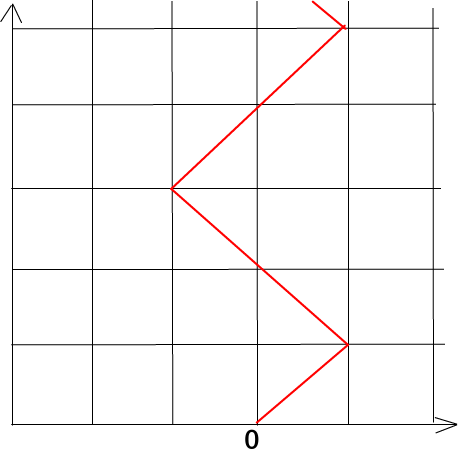
\includegraphics[width=.4\textwidth]{./pictures/13_8.png}
  \caption{Блуждание частицы}
  \label{fig:138}
\end{figure}

Найдём вероятность $P \left( \varlimsup \limits_{n \to \infty } A_{2n} \right) $.

Вероятность события $A_{2n}$ равна
$$P \left( A_{2n} \right) =
\left( \frac{2}{3} \cdot \frac{1}{3} \right)^n \cdot C_{2n}^n.$$

Ряд составленный из таких вероятностей
$$ \sum \limits_{n=1}^{ \infty } \left( \frac{2}{3} \cdot \frac{1}{3} \right)^n \cdot C_{2n}^n =
\sum \limits_{n=1}^{ \infty } \left( \frac{2}{9} \right)^n \cdot \frac{ \left( 2n \right)!}{n!n!}.$$

По формуле Стирлинга
$$n! \sim \frac{ \sqrt{2 \pi n} n^n}{\exp{n}}.$$
Подставим эту формулу в вероятность
\begin{equation*}
\begin{split}
P \left( A_{2n} \right) \sim
\left( \frac{2}{9} \right)^n \cdot
\frac{ \sqrt{2 \pi n}}{ \sqrt{2 \pi n} \sqrt{2 \pi n}} \cdot \frac{ \left( 2n \right)^{2n}}{n^n n^n} \cdot
\frac{\exp{n} \cdot \exp{n}}{ \exp{2n}} = \\
= \left( \frac{2}{9} \right)^n \cdot \frac{2}{2 \sqrt{ \pi n}} \cdot \frac{ \left( 2n \right)^{2n}}{n^{2n}} =
\left( \frac{2}{9} \right)^n \cdot \frac{2^{2n}}{ \sqrt{ \pi n}} =
\frac{2^n \cdot 2^{2n}}{9^n \sqrt{ \pi n}} =
\frac{2^{3n}}{9^n \sqrt{ \pi n}} = \\
= \left( \frac{2^3}{9} \right)^n \cdot \frac{1}{ \sqrt{ \pi n}} =
\left( \frac{8}{9} \right)^n \cdot \frac{1}{ \sqrt{ \pi n}}.
\end{split}
\end{equation*}
Ряд сходится.
Отсюда следует, что $P \left( \varlimsup \limits_{n \to \infty } A_{2n} \right) = 0$.


\addcontentsline{toc}{section}{Дополнительные задачи}
\section*{Дополнительные задачи}

\addcontentsline{toc}{section}{Домашнее задание}
\section*{Домашнее задание}

\subsubsection*{13.14}

\textit{Задание.} Найдите вероятность того, что при последовательных подбрасываниях игрального кубика серия очков 1, 2, 3, 4, 5, 6 встретится конечное количество раз.

\textit{Решение.}
Рассмотрим события $A_1 =$ \{серия очков 1, 2, 3, 4, 5, 6 выпадет при подбрасываниях 1 --- 6\},
$A_2 =$ \{серия очков 1, 2, 3, 4, 5, 6 выпадет при подбрасываниях 7 --- 12\},
$ \dotsc, \, A_n =$ \{серия очков 1, 2, 3, 4, 5, 6 выпадет при подбрасываниях $6(n-1)+1$ --- $6n$\}.

Хотим доказать, что ряд из вероятностей таких событий расходится.
Для этого нужно посчитать вероятность такого события.
Подбрасывания независимы
$$P \left( A_k \right) =
\left( \frac{1}{6} \right)^6,$$
так как всего есть $ \left| \Omega \right| = 6^6$ вариантов выпадения очков при подбрасывании игрального кубика с шестью элементами 6 раз
(на каждой из шести позиций может стоять любая из шести цифр),
а серия 1, 2, 3, 4, 5, 6 только одна.
Ряд из таких вероятностей
$$ \sum \limits_{k=1}^{ \infty } P \left( A_k \right) =
\sum \limits_{k=1}^{ \infty } \left( \frac{1}{6} \right)^6 =
+ \infty \left( \frac{1}{6} \right)^6 =
+ \infty.$$

По второй части леммы Бореля-Кантелли для независимых
$$A_1, A_2, \dotsc, A_n \in \mathcal{F},$$
если
$$ \sum \limits_{n=1}^{ \infty } P \left( A_n \right) =
+ \infty $$
(ряд, составленный из вероятностей расходится), то $P \left( \varlimsup \limits_{n \to \infty } A_n \right) = 1$.
Нас интересует обратное событие,
то есть
$$P \left( \varliminf \limits_{n \to \infty } A_n \right) =
P \left( \overline{ \varlimsup \limits_{n \to \infty } A_n} \right) =
1 - P \left( \varlimsup \limits_{n \to \infty } A_n \right) =
1 - 1 =
0.$$

\subsubsection*{13.15}

\textit{Задание.} Пусть $ \left\{ \xi_n \right\}_{n \geq 1}$ --- последовательность независимых случайных величин.
Найдите вероятность $P \left( \varliminf \limits_{n \to \infty } \xi_n = 0 \right) $, если:
\begin{enumerate}[label=\alph*)]
\item $P \left( \xi_n = 0 \right) = P \left( \xi_n = 1 \right) = 1/2$;
\item $P \left( \xi_n = 1/n \right) = P \left( \xi_n = 1 \right) = 1/n, \, P \left( \xi_n = 2 \right) = 1 - 2/n$;
\item $P \left( \xi_n = 0 \right) = 1/2^n, \, P \left( \xi_n = 1 \right) = 1 - 1/2^n$.
\end{enumerate}

\textit{Решение.}
\begin{enumerate}[label=\alph*)]
\item Нужно показать,
что в последовательности $ \xi_1, \xi_2, \dotsc, \xi_n, \dotsc $ бесконечно много нулей и $P \left( A_n \right.$ бесконечно часто) $= 1$,
где $A_n = \left\{ \xi_n = 0 \right\} $.
Эти события независимы, потому что $ \left\{ \xi_n \right\}_{n \geq 1}$ --- независимы.
Их вероятность по условию равна
$$P \left( A_n \right) =
\frac{1}{2}.$$
Рассмотрим ряд
$$ \sum \limits_{n=1}^{ \infty } P \left( A_n \right) =
\sum \limits_{n=1}^{ \infty } \frac{1}{2} =
+ \infty.$$
Тогда по второй части леммы Бореля-Кантелли $P \left( \varliminf \limits_{n \to \infty } \xi_n = 0 \right) = 1$;
\item нужно показать,
что в последовательности $ \xi_1, \xi_2, \dotsc, \xi_n, \dotsc $ бесконечно много нулей и $P \left( A_n \right.$ бесконечно часто) $= 1$,
где
$$A_n =
\left\{ \xi_n < \frac{1}{N} \right\}.$$
Эти события независимы, потому что $ \left\{ \xi_n \right\}_{n \geq 1}$ --- независимы.
По условию
$$P \left( \xi_n = \frac{1}{n} \right) =
\frac{1}{n}.$$
Рассмотрим ряд
$$ \sum \limits_{n=1}^{ \infty } P \left( A_n \right) \geq
\sum \limits_{n=1}^{ \infty } \frac{1}{n} =
+ \infty.$$
Тогда по второй части леммы Бореля-Кантелли $P \left( \varliminf \limits_{n \to \infty } \xi_n = 0 \right) = 1$;
\item нужно показать,
что в последовательности $ \xi_1, \xi_2, \dotsc, \xi_n, \dotsc $ бесконечно много нулей и $P \left( A_n \right.$ бесконечно часто) $= 1$,
где $A_n = \left\{ \xi_n = 0 \right\} $.
Вероятность этих событий по условию равна
$$P \left( A_n \right) =
\frac{1}{2^n}.$$
Рассмотрим ряд
$$ \sum \limits_{n=1}^{ \infty } P \left( A_n \right) =
\sum \limits_{n=1}^{ \infty } \frac{1}{2^n} =
\frac{ \frac{1}{2}}{1 - \frac{1}{2}} =
1.$$
Тогда по первой части леммы Бореля-Кантелли $P \left( \varliminf \limits_{n \to \infty } \xi_n = 0 \right) = 0$.
\end{enumerate}

\subsubsection*{13.16}

\textit{Задание.} Пусть для последовательности событий $ \left\{ A_n \in \mathcal{F} \right\}_{n \geq 1}$ существует событие $A \in \mathcal{F}$ такое, что
$$ \sum \limits_{i=1}^{ \infty } P \left( A \cap A_i \right) < + \infty.$$
Докажите, что $P \left( \varlimsup \limits_{n \to \infty } A_n \right) \leq 1 - P \left( A \right) $.

\textit{Решение.} По первой части леммы Бореля-Кантелли из того, что
$$ \sum \limits_{i=1}^{ \infty } P \left( A \cap A_i \right) < + \infty $$
следует, что $P \left( \varlimsup \limits_{n \to \infty } \left( A \cap A_n \right) \right) = 0$.
Можем вынести $A$ из-под знака предела
$P \left( \varlimsup \limits_{n \to \infty } \left( A \cap A_n \right) \right) =
P \left( A \cap \varlimsup \limits_{n \to \infty } A_n \right) =
0$.
События не пересекаются,
значит
$P \left( \varlimsup \limits_{n \to \infty } A_n \right) =
P \left( \varlimsup \limits_{n \to \infty } A_n \setminus A \right) =
P \left( \varlimsup \limits_{n \to \infty } A_n \cap \overline{A} \right) \leq
P \left( \overline{A} \right) = \\
= 1 - P \left( A \right) $.

\subsubsection*{13.17}

\textit{Задание.}
На вероятностном пространстве
$ \left( \Omega, \mathcal{B}, P \right) $, где $ \Omega = \left( 0, 1 \right), \, \mathcal{B} = \\
= \mathcal{B} \left( \left( 0, 1 \right) \right), \, P$ ---
мера Лебега, рассмотрим последовательность событий
$$ \left\{ A_n = \left( 0, \frac{1}{n} \right) \right\}_{n \geq 1}.$$
Покажите, что
$$ \sum \limits_{n=1}^{ \infty } P \left( A_n \right) =
\infty,$$
но $P \left( A_n \right.$ бесконечно часто) $= 0$.

\textit{Решение.}
Вероятность задана как мера Лебега,
то есть расстояние между точками
$$P \left( A_n \right) =
P \left[ \left( 0, \frac{1}{n} \right) \right] =
\frac{1}{n} - 0 =
\frac{1}{n}.$$
Ряд, составленный из таких вероятностей расходится (он гармонический), т.е.
$$ \sum \limits_{n=1}^{ \infty} P \left( A_n \right) =
\sum \limits_{n=1}^{ \infty } \frac{1}{n} =
+ \infty.$$

Найдём верхний предел
$$ \varlimsup \limits_{n \to \infty } A_n =
\bigcap \limits_{n=1}^{ \infty } \bigcup \limits_{m=n}^{ \infty } \left( 0, \frac{1}{m} \right) =
\left( 0, 0 \right),$$
так как объединение таких интервалов даёт
$$ \left( 0, \frac{1}{m} \right),$$
а пересечение --- $ \left( 0, 0 \right) $.

Вероятность этого предела равна
$P \left( A_n \right.$ бесконечно часто) $=$
$$= P \left( \varlimsup \limits_{n \to \infty } A_n \right) =
P \left[ \left( 0, 0 \right) \right] =
0 - 0 =
0.$$

\subsubsection*{13.18}

\textit{Задание.}
Рассмотрим последовательность независимых экспериментов,
в каждом из которых некоторое событие --- успех --- происходит с вероятностью $p$, а противоположное событие --- неудача --- с вероятностью $q = 1 - p$.
Пусть $A_n$ --- событие, которое состоит в том, что между $2^n$-ым и $2^{n+1}$-ым экспериментами произойдёт серия из $n$ последовательных успехов.
Докажите, что если
$$p \geq \frac{1}{2},$$
то с вероятностью 1 произойдёт бесконечно много событий $A_n$, а если
$$p < \frac{1}{2},$$
то с вероятностью 1 произойдёт только конечное количество $A_n$.

\textit{Решение.} Нужно показать, что при
$$p \geq \frac{1}{2}$$
вероятность $P \left( A_n \right.$ бесконечно часто) $= 1$, то есть $P \left( \varlimsup \limits_{n \to \infty } A_n \right) = 1$, а при
$$p < \frac{1}{2}$$
вероятность $P \left( A_n \right.$ произошло конечное число раз) $= 0$, то есть
$$P \left( \varliminf \limits_{n \to \infty } A_n \right) = 1.$$

По лемме Бореля-Кантелли для первого случая надо показать, что ряд, составленный из вероятностей расходится, а для второго --- сходится.
Найдём вероятность события $A_n$.
Выбираем $n$ событий из $2^n$, которые окажутся успешными.
Тогда вероятность равна
$$P \left( A_n \right) =
C_{2^n}^n p^n \left( 1 - p \right)^{2^n-n}.$$

\subsubsection*{13.20}

\textit{Задание.} Пусть $ \left\{ \xi_n \right\}_{n \geq 1}$ --- последовательность независимых одинаково распределённых случайных величин с функцией распределения
$$F \left( x \right) =
\begin{cases}
0, \qquad x < 1, \\
1 - \frac{1}{x}, \qquad x \geq 1.
\end{cases}$$
 
\textit{Решение.} Знаем, что
$$P \left( \xi_n \leq x \right) =
F \left( x \right) =
\begin{cases}
0, \qquad x < 1, \\
1 - \frac{1}{x}, \qquad x \geq 1.
\end{cases}$$

Хотим доказать, что
$$P \left( \varlimsup \limits_{n \to \infty } \frac{ \xi_n}{ \sqrt{n}} =
+ \infty \right) =
1.$$

Есть некоторая подпоследовательность, которая сходится к бесконечности.

Начнём с вероятности
$$P \left( \frac{ \xi_n}{ \sqrt{n}} > \sqrt{n} \right).$$
Если покажем, что ряд
$$ \sum \limits_{n=1}^{ \infty } P \left( \frac{ \xi_n}{ \sqrt{n}} > \sqrt{n} \right) =
+ \infty,$$
по условию $ \left\{ \xi_n \right\}_{n \geq 1}$ --- независимы, то $P \left( \xi_n / \sqrt{n} > \sqrt{n} \right.$ бесконечно часто $ \left. \right) = 1$.
Отсюда следует, что
$$P \left( \frac{ \xi_n}{ \sqrt{n}} > \sqrt{n} \right) = P \left( \xi_n > n \right) = 1 - P \left( \xi_n \leq n \right).$$

Знаем, что $P \left( \xi_n \leq n \right) $ --- функция распределения
$$P \left( \frac{ \xi_n}{ \sqrt{n}} > \sqrt{n} \right) =
1 - P \left( \xi_n \leq n \right) =
1 - F \left( n \right) =
1 - \left( 1 - \frac{1}{n} \right) =
\frac{1}{n}.$$
Отсюда следует, что ряд расходящийся
$$ \sum \limits_{n=1}^{ \infty } P \left( \frac{ \xi_n}{ \sqrt{n}} > \sqrt{n} \right) =
+ \infty,$$
по условию $ \left\{ \xi_n \right\}_{n \geq 1}$ --- независимы.
Отсюда следует, что $P \left( \xi_n / \sqrt{n} > \sqrt{n} \right.$ бесконечно часто $ \left. \right) = 1$.
Отсюда следует, что
$$P \left( \varlimsup \limits_{n \to \infty } \frac{ \xi_n}{ \sqrt{n}} =
+ \infty \right) =
1.$$

\subsubsection*{13.21}

\textit{Задание.} На отрезке $ \left[ 0, 1 \right] $ последовательно выбирают наугад точки
$$A_1, A_2, \dotsc.$$
Пусть $ \rho_n$ является минимальным из расстояний от точек $A_1, \dotsc, A_n$ к фиксированной точке $A$ на отрезке $ \left[ 0, 1 \right] $.
Доказать, что $P \left( \rho_n \to \left( n \to \infty \right) 0 \right) = 1$.

\textit{Решение.} Пусть $d_i = dist \left( A, A_i \right) $.

Положим $ \rho_n = \min \left( d_1, \dotsc, d_n \right) $.

Хотим показать, что $P \left( \rho_n \to \left( n \to \infty \right) 0 \right) = 1$.

Начиная с некоторого номера $ \forall \epsilon > 0 \, \exists N \, \forall n \geq N, \qquad \rho_n < \epsilon $ --- определение сходимости к нулю.

Пусть $ \epsilon $ --- произвольное как угодно малое число, $ \epsilon > 0$.
Рассмотрим событие
$P \left( \rho_n > \epsilon \right) =
P \left( \min \left( d_1, \dotsc, d_n \right) > \epsilon \right) =
P \left( d_1 > \epsilon, d_2 > \epsilon, \dotsc, d_n > \epsilon \right) $.
Воспользуемся независимостью
$$P \left( d_1 > \epsilon, d_2 > \epsilon, \dotsc, d_n > \epsilon \right) =
P \left( d_1 > \epsilon \right) \cdot \dotsc \cdot P \left( d_n > \epsilon \right).$$
Рассмотрим рисунок \ref{fig:1321}.
На нём область, отмеченная красным --- место, куда должна попасть точка $A_i$.

\begin{figure}[h!]
  \centering
  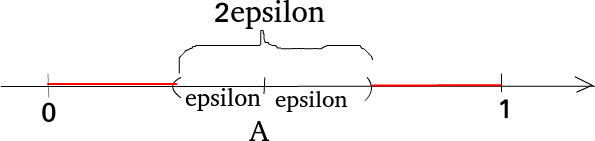
\includegraphics[width=.4\textwidth]{./pictures/13_21.png}
  \caption{Область, куда может попасть точка}
  \label{fig:1321}
\end{figure}

Из рисунка $P \left( d_1 > \epsilon \right) \cdot \dotsc \cdot P \left( d_n > \epsilon \right) = \left( 1 - 2 \epsilon \right)^n = r^n, r < 1$.
Из этого следует, что если рассмотрим ряд, составленные из этих вероятностей, получим
$$ \sum \limits_{n=1}^{ \infty } P \left( \rho_n > \epsilon \right) = \sum \limits_{n=1}^{ \infty } r^n = \frac{r}{1-r} = \frac{1-2 \epsilon }{2 \epsilon } < + \infty.$$

Ряд сходящийся.
Отсюда следует, что $P \left( \left( \rho_n > \epsilon \right) \right.$ происходит бесконечно часто) $= 0$.

Это значит, что $ \forall N \, \exists n > N, \qquad \left( \rho_n > \epsilon \right) $ выполняется.

Вероятность такого события равна нулю.

Противоположное событие означает
$$P \left( \exists N \, \forall n > N, \qquad \left( \rho_n < \epsilon \right) \right) =
1 =
P \left( \left( \rho_n < \epsilon \right) \right.$$
для всех $n$, начиная с некоторого номера) --- это то, что хотели показать.
